

%%% AAAI PRESENTATION BELOW
\begin{frame}{Learning a causal model}
\includegraphics[width=\linewidth]{causal_figures/conceptA}
\begin{itemize}
\item Our initial goal was how to learn a causal model in a reinforcement-learning setting
\end{itemize}
\end{frame}

\begin{frame}{What is a causal model?}%\only<3->{ \osvg{whatis} }
\begin{itemize}
\item How Nature assigns the variables \pause
\end{itemize}
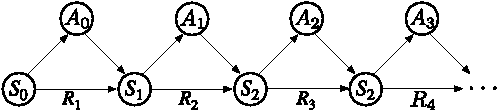
\includegraphics[width=\linewidth]{causal_figures/sutton2018_79}
\begin{itemize} 
\item The Markov decision process? 
\end{itemize}
\end{frame}

\begin{frame}%{What is a causal model?}
\begin{description}%\osvg{chess}
\item[Chess] \emph{"Playing passively caused me to loose"} \pause \pause
\item[Control] \emph{"Bicycling at the edge of the road caused me to loose control"} \pause 
\item[Social science] \emph{"Studying harder caused an increase in grades"} \pause
\end{description}
\end{frame}
\begin{frame}{Problem formulation}%\osvg{problem}
\begin{figure}
\centering
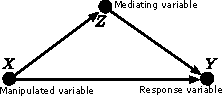
\includegraphics[width=1.0\linewidth]{causal_figures/medanal1}
\end{figure}

\begin{itemize}
\item How to learn a parsimonious causal model in a reinforcement learning setting? \pause
\begin{itemize} 
\item Explain outcome variable $Y$ \pause
\item Include our choice in behavior $X$  \pause
\begin{itemize}
	\item Baseline policy $\pi_a$ 
	\item Alternative policy $\pi_b$
\end{itemize}
\item A learned variable $Z$ affected by policy and which affect the outcome $Y$ \pause
\end{itemize}
\item Under-determined problem (many choices of $Z$!) \pause
\item Causal model is \redt{descriptive} rather than \redt{generative} 
\end{itemize}
\end{frame}

\begin{frame}{Our approach}
	\begin{itemize}
\item Assume we are given a baseline policy $\pi_a$ \pause
\item The variable $Z$ should be associated with a high reward 
$$
\EE[Y | Z=1] > \EE[Y | Z=0]
$$ \pause
\item Policy choice $\pi_a$ vs. $\pi_b$ should influence $Z$ \pause
\item This trade-of is naturally realized by the \redt{natural indirect effect}~\citep{pearl2001direct}
\begin{align*}
	\NIE & = \left( \EE\left[Y | Z=1, \pi_a \right] - \EE\left[Y | Z=0, \pi_a \right] \right)  \\  
	& \times  \left( P(Z=1| \pi_b) -P(Z=1| \pi_a) \right).%\label{eq12}
\end{align*} \pause
\item Simply determine $\pi_b^*, Z^* = \arg\,\max_{\pi_b, Z} \NIE$
	\end{itemize}
\end{frame}

\begin{frame}{Implementation: $Z$}
\begin{itemize}
\item We model $Z$ as a stopping process:
\begin{align*}
	Z = \max\{Z_0, Z_1, \dots Z_T\}.
\end{align*}	
\item Each $Z_t \in \{0,1\}$ are parameterized using a neural network
$$
Z_t \sim \textrm{Bern}(\Phi(s_t))
$$
\end{itemize}
\end{frame}

\begin{frame}{Implementation: Policy}
\begin{figure}
	\centering
	\includegraphics[width=0.7\linewidth]{causal_figures/medanal2}
\end{figure}

	\begin{itemize}
	\item The combined policy will either follow $\pi_a$, or follow an alternative policy $\pi_b$ until $Z$ is true after which it follows $\pi_a$. 
\begin{align*}
	\pi = \begin{cases} \pi_a & \mbox{if $\Pi = a$ } \\ \left(1-\max\{Z_{0}, \dots, Z_t\} \right)\pi_b +\max\{Z_{0}, \dots, Z_t\} \pi_a
		& \mbox{if $\Pi = b$. }\end{cases} %\label{eq10}
\end{align*}
	\end{itemize}	
\end{frame}

\begin{frame}{Implementation: Maximization}
\begin{itemize}
	\item How to maximize the $\NIE$ wrt. $Z$ and $\pi_b$?
	\begin{align*}
		\NIE & = \left( \EE\left[Y | Z=1, \pi_a \right] - \EE\left[Y | Z=0, \pi_a \right] \right)  \\  
		& \times  \left( P(Z=1| \pi_b) -P(Z=1| \pi_a) \right).%\label{eq12}
	\end{align*} \pause
\item Let's first focus on simply estimating this quantity iteratively similar to the Bellman backup for the value function
$$
V(s_{t} ) = \EE[ R_{t+1} + \gamma V(s_{t+1}) | S_t=s_t]
$$
\end{itemize}
\end{frame}

\begin{frame}{Overview}
Define whether $Z=1$ after time step $t$:
\begin{align*}
	Z_t^\infty = \max\{Z_t,Z_{t+1}, \dots,\} %(1-Z_{k-1}) = \mbox{One of $Z_k,\dots$ is true and $Z_k$ is false}
\end{align*}  \pause
We will actually estimate:
\begin{align*}
	v^{\infty}_t(s_t) & = P(Z^\infty_t =1 | S_t=s_t, Z_{t-1} = 0), \\
	v^{z}_t(s_t) & = \EE\left[\sum_{k=0}^\infty \gamma^{k}R_{t+k+1} | S_t=s_t, Z_t^\infty = z, Z_{t-1} = 0\right].  %\label{eq19} 
\end{align*}
Note that $v^\infty_0(s_0) = P(Z = 1| s_0)$ and $v^z_0(s_0) = \EE[G_0 | s_0, Z=z]$. \pause
They satisfy recursions
\begin{subequations} 
\begin{align*}
		v^\infty_t(s_t) & = \Phi(s_t) + (1-\Phi(s_t) ) \EE\left[ v^\infty_{t+1}(S_{t+1} )| s_t\right],  \\ 
		v^{1}_t(s_t) & =  \frac{ V(s_t) \Phi(s_t) }{V_t^\infty(s_t) }  
		+ \frac{  1\!-\! \Phi(s_t)  }{V_t^\infty(s_t) } \EE\left[ v^\infty_{t+1}(S_{t+1}) \left( R_{t+1} + \gamma v^{1}_{t+1}(S_{t+1} ) \right) \mid s_t   \right], \nonumber \\	
\end{align*}
\end{subequations}
Both have the form
\begin{align*}
	v_t(s_t) & =\EE\left[H_t(s_t,S_{t+1})  + G_t(s_t, S_{t+1}) v_{t+1}(S_{t+1} )  )  \middle| s_t\right] %\label{eq22a}
\end{align*}\end{frame}

\begin{frame}
By applying the recursion $n$ times we get:
\begin{align*}  
	v_t(s_t) & =\EE\left[ \sum_{i=t}^{t+n-1} H_i \prod_{\ell=t}^{i-1} G_\ell + v_{t+n}(S_{t+n})  \prod_{\ell = t}^{ t+n-1} G_\ell   \middle| s_k\right], %\label{eq35}
\end{align*}
\begin{itemize}
	\item This can be estimated using a $V$-trace estimator~\citep{espeholt2018impala}
\end{itemize}
\begin{subequations}
	\begin{align*}
		V_t(s_t) &= v(s_t) + \sum_{i=t}^{t+n-1} \left( \prod_{\ell=t}^{i-1} c_\ell G_{\ell} \right)	\delta_i  \\
		\delta_i & = \rho_i \left[ H_i(s_i, s_{i+1}) + G_i v(S_{i+1})- v(S_i) \right]  
	\end{align*} %\label{eq22}
\end{subequations}
where $c_\ell$ and $\rho_k$ are truncated importance sampling weights: 
\begin{align*} 
	\rho_t = \min\left\{\bar \rho, \frac{\pi(a_t | s_t)  }{\mu(a_t | s_t) }  \right\},\
	c_t = \min\left\{\bar c, \frac{\pi(a_t | s_t)  }{\mu(a_t | s_t) }  \right\}, \nonumber
\end{align*}
\begin{itemize}
	\item Method converge in the tabular case when $0< \gamma < 1$ and $0 < \Phi(s) < 1$
\end{itemize}
\end{frame}

\begin{frame}{Summary:}
\begin{align*}
	\NIE & = \left( \EE\left[Y | Z=1, \pi_a \right] - \EE\left[Y | Z=0, \pi_a \right] \right)  \\  
	& \times  \left( P(Z=1| \pi_b) -P(Z=1| \pi_a) \right).%\label{eq12}
\end{align*}
\begin{itemize}
	\item Train a baseline policy $\pi_a$
\item Replace the terms $\EE\left[Y | Z=1, \pi_a \right]$ and $P(Z=1| \pi_b)$ by $n$-step $V$-trace estimates to obtain a concrete parameterizing in terms of behavior policy $\pi_b$ and $\Phi$. 
\item Optimize using SGD
\end{itemize}
\end{frame}

\begin{frame}{Example: two-stage environment}
\centering
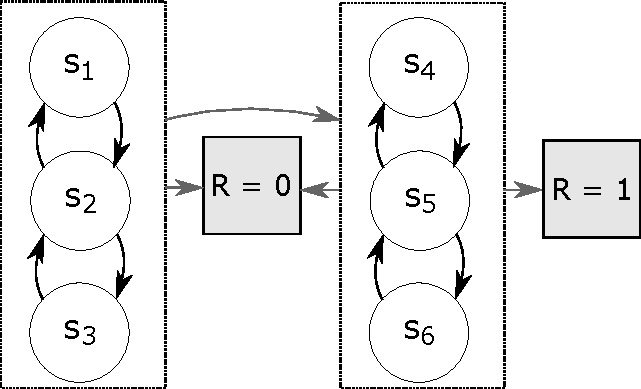
\includegraphics[width=.33\linewidth]{causal_figures/twostage}
$$
\NIE \propto  \EE\left[Y | Z=1, \pi_a \right] - \EE\left[Y | Z=0, \pi_a \right]  
$$ \pause
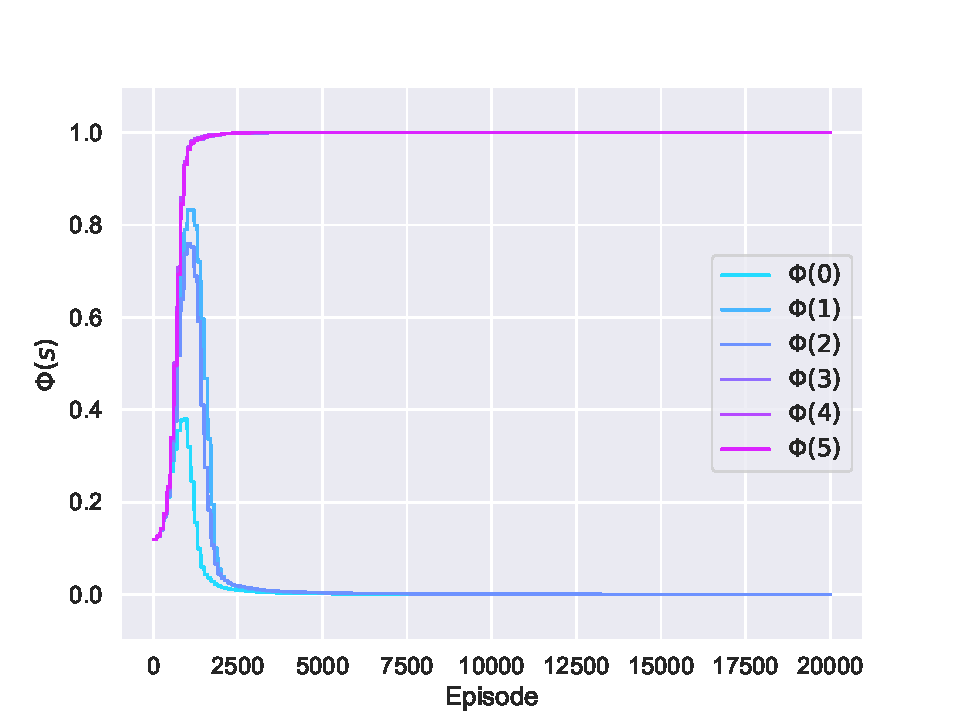
\includegraphics[width=.5\linewidth]{causal_figures/twostage_Phi}~
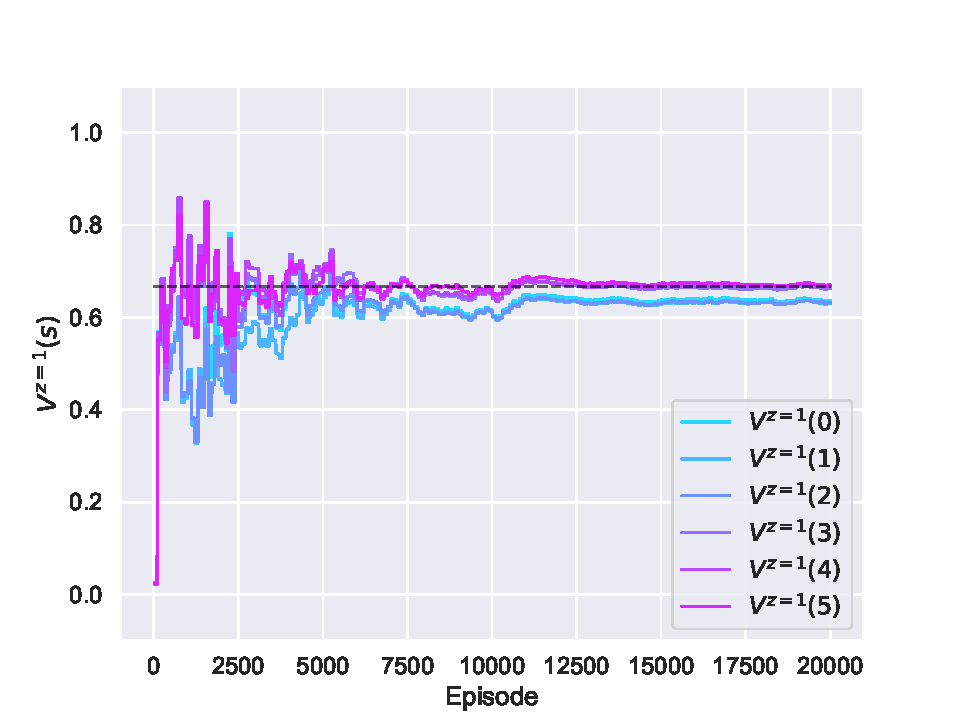
\includegraphics[width=.5\linewidth]{causal_figures/twostage_Vz1}
\end{frame}
\begin{frame}{Example: Doorkey environment}
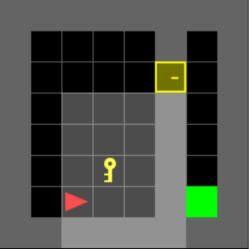
\includegraphics[width=.33\linewidth]{causal_figures/doorkey}~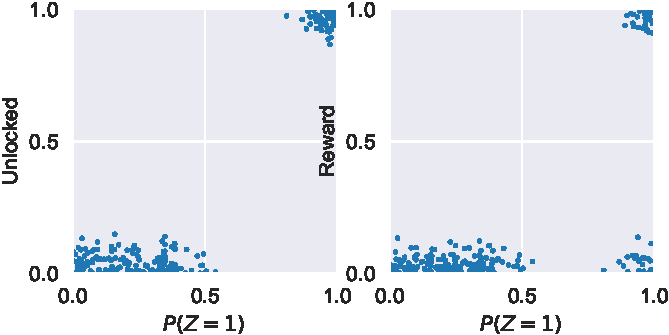
\includegraphics[width=0.66\linewidth]{causal_figures/scatter_AB}
\begin{itemize}
	\item Trained on a  small Doorkey environment
	\item Learned variable $Z$ corresponds to unlocking the door 
\end{itemize}
\end{frame}

\begin{frame}\frametitle{Causality and optimal policies?}
\begin{align*}
	\NIE & = \left( \EE\left[Y | Z=1, \pi_a \right] - \EE\left[Y | Z=0, \pi_a \right] \right)  \\  
	& \times  \left( P(Z=1| \pi_b) -P(Z=1| \pi_a) \right).%\label{eq12}
\end{align*}
\begin{itemize}
\item The NIE will generally not be large when $\pi_a$ is optimal\pause
\item How well-defined is the notation of a parsimonious causal model when an optimal policy is known? 
\end{itemize}		
\vspace{3cm}
\only<2->{\osvg{chess2} }
\end{frame}


%
%\begin{frame}\begin{itemize}        
%    \item Our problem becomes: Learn the coarse-grained graph. Picture of Doorkey graph. 
%\end{itemize}\end{frame}\begin{frame}\begin{itemize}
%        \item Slide: Relationship to RL. Example of coarse grained vairables: $\pi \rightarrow R$. We adopt this to include new variable $Z$
%        \item Discussion of minimal elements in the graph. Reward, and choice of policy. We must include a choice of policy because no single action result in $Z$ (as we think about Z)
%\end{itemize}
%\end{frame}
%
%\begin{frame}\begin{itemize}        
%        \item Learning a variable such as $Z$ involves trade-off (what it means to be acausal variable). Must be somthing that the agent can archive, must be reasonable hard to archive (at least not be impollied by current behavior), and most affect reward. The NIE archive this tradeof
%    \end{itemize}\end{frame}\begin{frame}\begin{itemize}
%        \item Examples of situations the NIE exludes ($Z=R$)
%        \end{itemize}\end{frame}\begin{frame}\begin{itemize}
%        \item Estimation of the NIE using Bellman updates
%\end{itemize}
%\end{frame}
%
%\begin{frame}\begin{itemize}
%        \item Example using two-stage. Pictyre of Twostage to root it. 
%    \end{itemize}\end{frame}\begin{frame}\begin{itemize}
%        \item Example using Doorkey
%        \end{itemize}\end{frame}\begin{frame}\begin{itemize}
%        \item Implications: coarse-grained variable in our framework can only be found if the alterantive, base-line policy is not optimal. The question is if this is a defect or a general feature of coarse-rgained causal learning. 
%    \end{itemize}
%\end{frame}
%    
%
%\begin{frame}{Example}
%\begin{figure}\centering
%	\includegraphics[width=0.9\linewidth]{causal_figures/conceptA}	
%	\caption{In \doorkey, the agent (red) must learn to pick up the key to open the door and get to the goal. }
%\end{figure}
%\end{frame}
%
%\begin{frame}{Mediation analysis}
%
%\begin{figure}
%	\centering
%	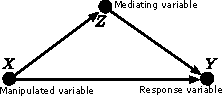
\includegraphics[width=1.0\linewidth]{causal_figures/medanal1}
%\end{figure}
%
%\begin{align}
%	\NIE_{x \rightarrow x'}(Y) = \sum_z \EE\left[Y | x,z\right][ P(z | x') - P(z | x)].%\label{eqNIE}
%\end{align}
%
%\end{frame}
%
%\begin{frame}{Frame Title}
%    \begin{figure}
%	\centering
%	\includegraphics[width=0.5\linewidth]{causal_figures/medanal2}
%\end{figure}
%
%\begin{align}
%	\pi = \begin{cases} \pi_a & \mbox{if $\Pi = a$ } \\ \left(1-Z_{0:t} \right)\pi_b +Z_{0:t} \pi_a
%		& \mbox{if $\Pi = b$. }\end{cases} \label{eq10}
%\end{align}
%
%
%\begin{align}
%	\NIE & = \left( \EE\left[Y | Z=1, \pi_a \right] - \EE\left[Y | Z=0, \pi_a \right] \right) \nonumber \\
%	&\quad  \times  \left( P(Z=1| \pi_b) -P(Z=1| \pi_a) \right).\label{eq12}
%\end{align}
%\end{frame}
%
%\begin{frame}{Bellman equations and tabular case}
%
%\begin{align}
%	v^{\infty}_t(s_t) & = P(Z^\infty_t =1 | S_t=s_t, Z_{t-1} = 0), \label{eq18} \\
%	v^{z}_t(s_t) & = \EE[G_t | S_t=s_t, Z_t^\infty = z, Z_{t-1} = 0].  \label{eq19} 
%\end{align}
%
%\begin{align}
%	V(s) & \underset{\alpha }{\leftarrow } r + \gamma V(s') \nonumber  \\% \label{eq35a} \\
%	V^\infty(s) & \underset{\alpha}{\leftarrow } \Phi(s)  + (1-\Phi(s) ) V^\infty(s') \label{eq35b} \\ 
%	%V^z(s_t) & \underset{a}{\leftarrow }  \frac{ V(s_t)  \Phi(s_t) }{ V^\infty(s_t) } + \frac{ 1 - \Phi(s_t) }{ V^\infty(s_t) } V^\infty(s_{t+1} )  r_{t+1}  + \frac{ 1 - \Phi(s_t) }{ V^\infty(s_t)  }  V^\infty(s_{t+1} )   \gamma V^z(s_{t+1} ) \\
%	%\!\!V^{1}(s) & \underset{\alpha}{\leftarrow }  
%	%\frac{ 
%	% V(s_t) \Phi(s_t)\! +\! (1\! -\! \Phi(s_t) )V^\infty(s_{t+1} ) \left(  r_{t+1}\! +\!  \gamma V^{1}(s_{t+1} )  \right) }{ V^\infty(s_t) } \label{eq35c} \\
%	\!\!V^{1}(s) & \underset{\alpha}{\leftarrow }  
%	\frac{ 
%		V(s) \Phi(s)\! +\! (1\! -\! \Phi(s) )V^\infty(s_{t} ) \left(  r\! +\!  \gamma V^{1}(s' )  \right) }{ V^\infty(s) } \nonumber %\label{eq35c}
%\end{align}
%    
%\end{frame}
%
%\begin{frame}{Results - tabular}
%\begin{figure}
%	\centering
%%	\subcaptionbox{\label{fig:twostage_a}}
%	{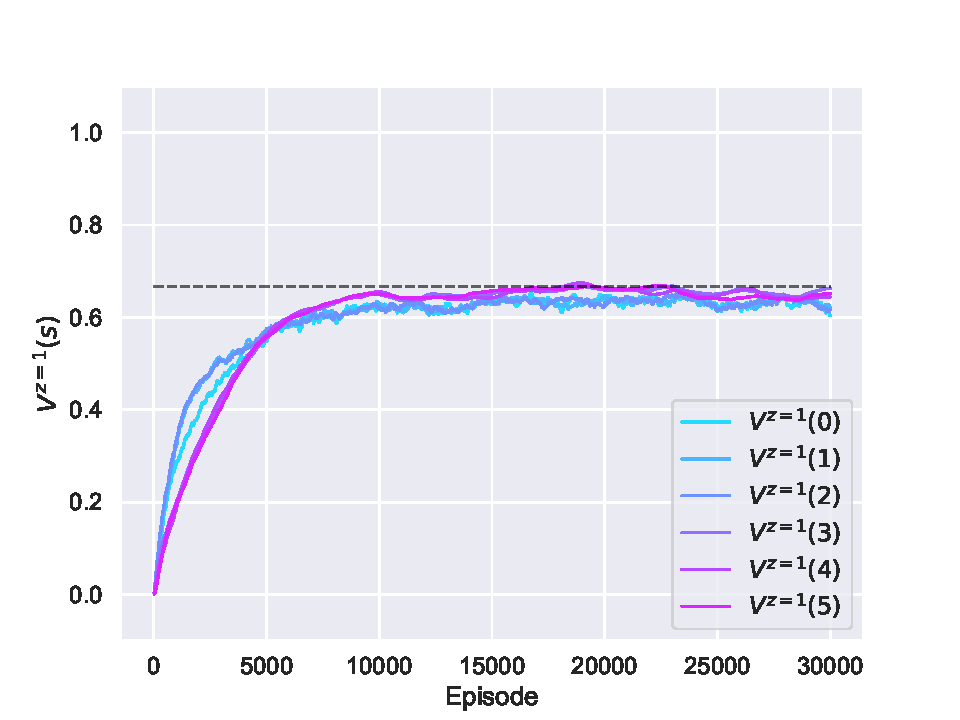
\includegraphics[width=.48\linewidth]{causal_figures/twostage_tabular_Vz1}}
%%	\subcaptionbox{\label{fig:twostage_b}}
%	{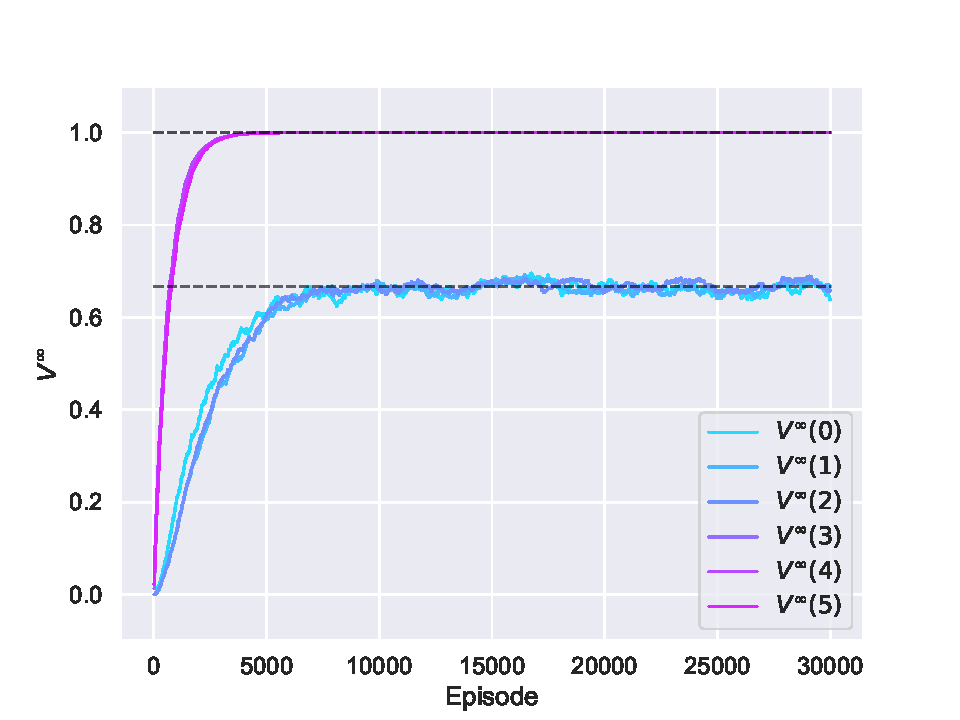
\includegraphics[width=.48\linewidth]{causal_figures/twostage_tabular_Vinf}}
%	%\caption{ (a-b) Trace plots of $v^{1}$ and $v^{\infty}$ for the tabular \twostage environment obtained using \cref{eq35}, with a given $\Phi$. (c-f) Estimates with neural function approximators for the value functions in the \twostage environment, while $\Phi$ is being learned.}
%\end{figure}    
%\end{frame}
%
%\begin{frame}{Results - neural}
%
%\begin{figure}
%	\centering
%%	\subcaptionbox{\label{fig:twostage_c}}
%	{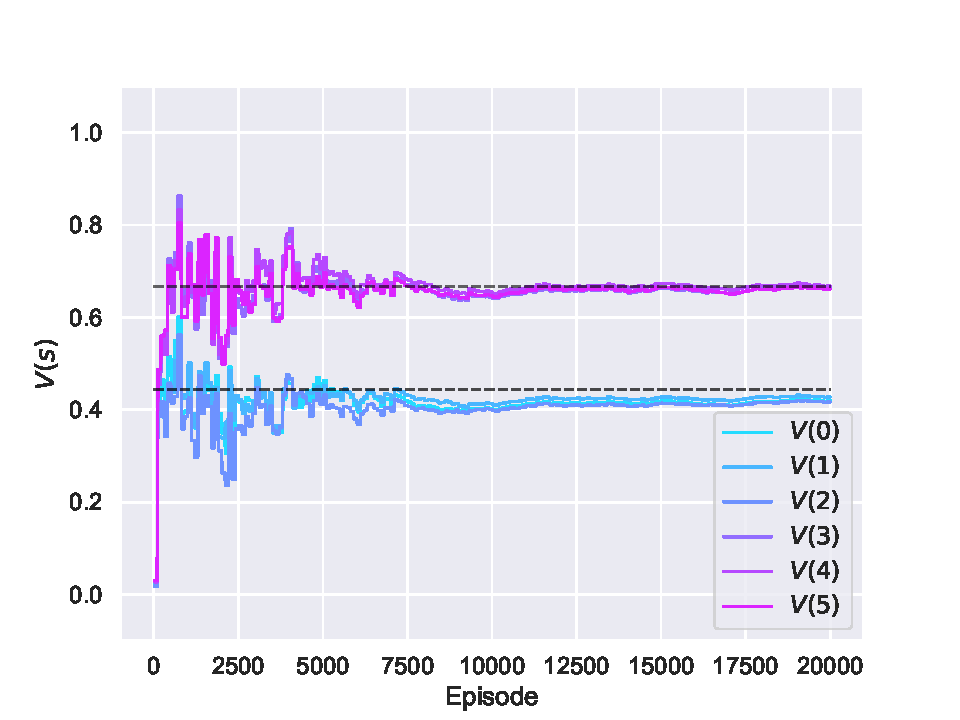
\includegraphics[width=.48\linewidth]{causal_figures/twostage_V}}
%%	\subcaptionbox{\label{fig:twostage_d}}
%	{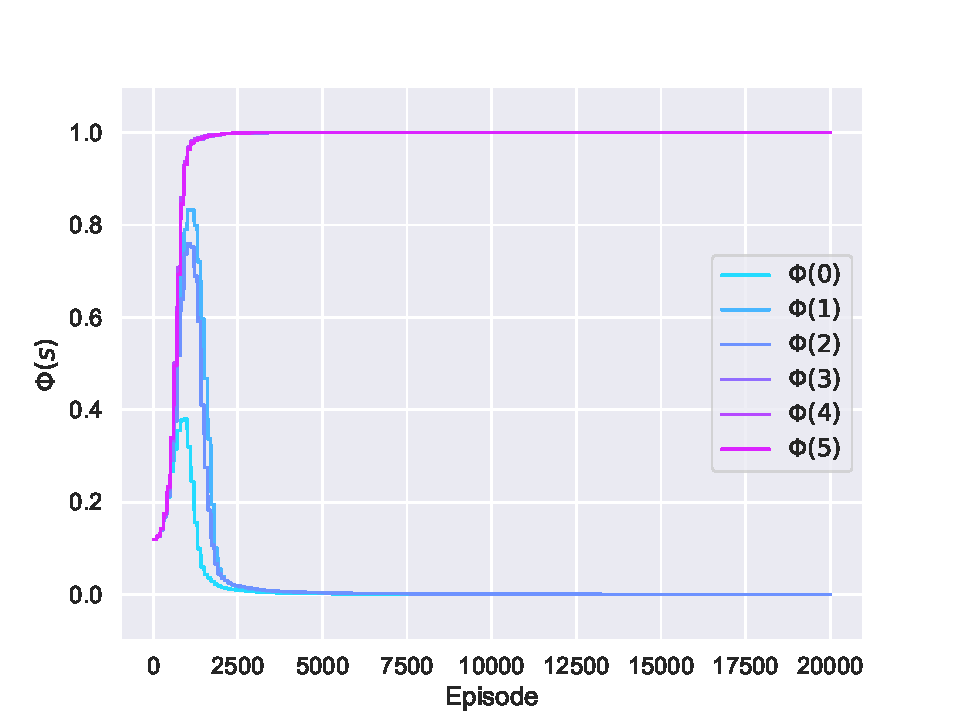
\includegraphics[width=.48\linewidth]{causal_figures/twostage_Phi}}
%%	\subcaptionbox{\label{fig:twostage_e}}
%	{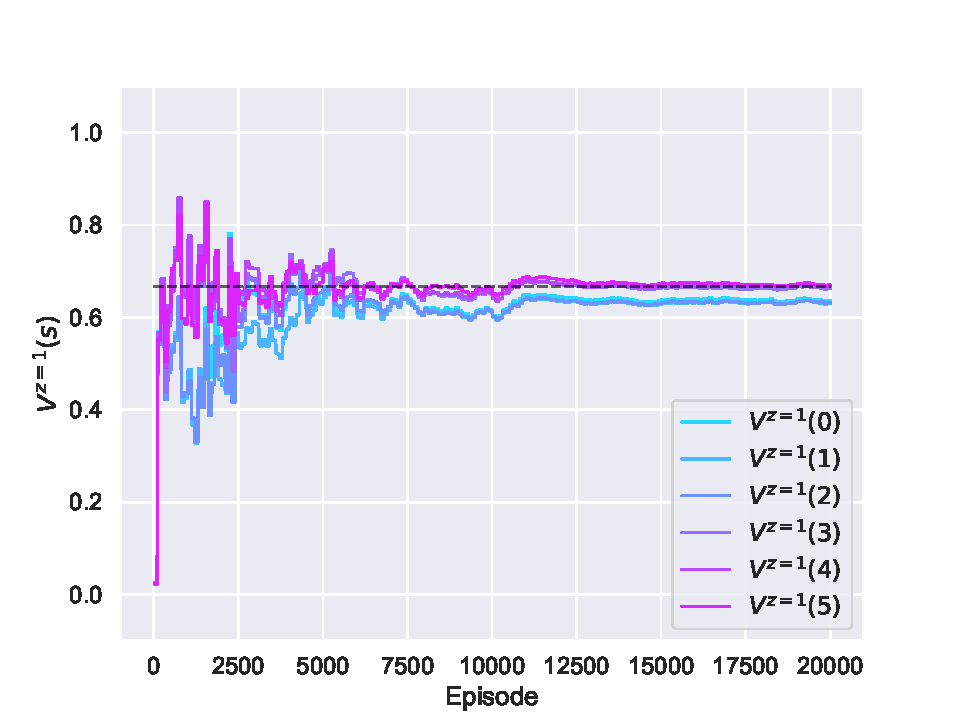
\includegraphics[width=.48\linewidth]{causal_figures/twostage_Vz1}}
%%	\subcaptionbox{\label{fig:twostage_f}}
%	{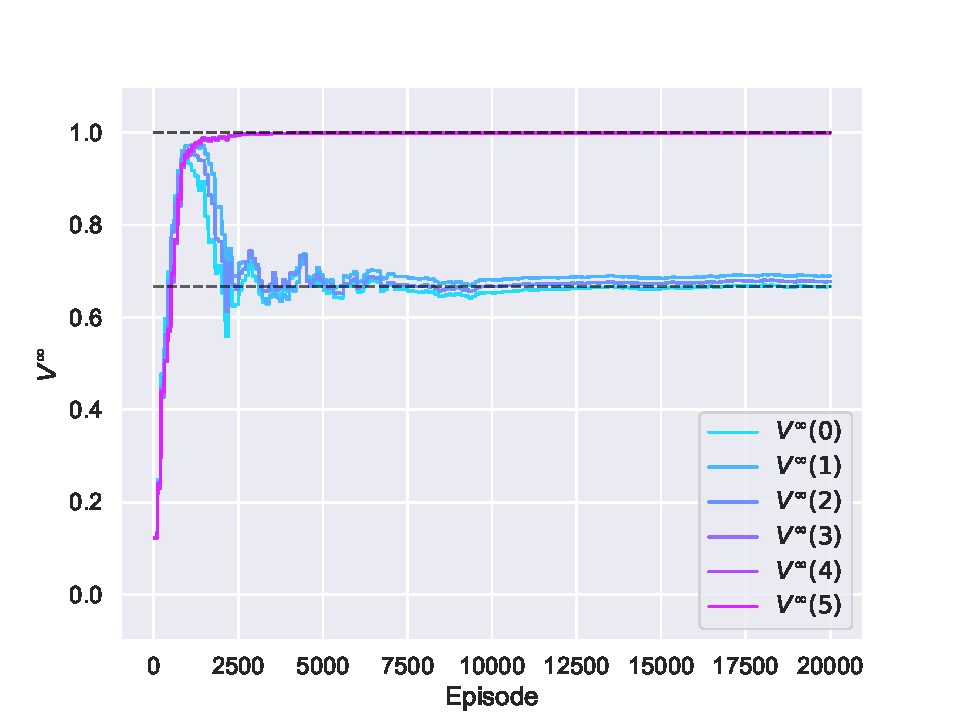
\includegraphics[width=.48\linewidth]{causal_figures/twostage_Vinf}}
%	%\caption{ (a-b) Trace plots of $v^{1}$ and $v^{\infty}$ for the tabular \twostage environment obtained using \cref{eq35}, with a given $\Phi$. (c-f) Estimates with neural function approximators for the value functions in the \twostage environment, while $\Phi$ is being learned.}
%\end{figure}    
%\end{frame}
%
%\begin{frame}{Representation}
%
%\begin{figure}
%	%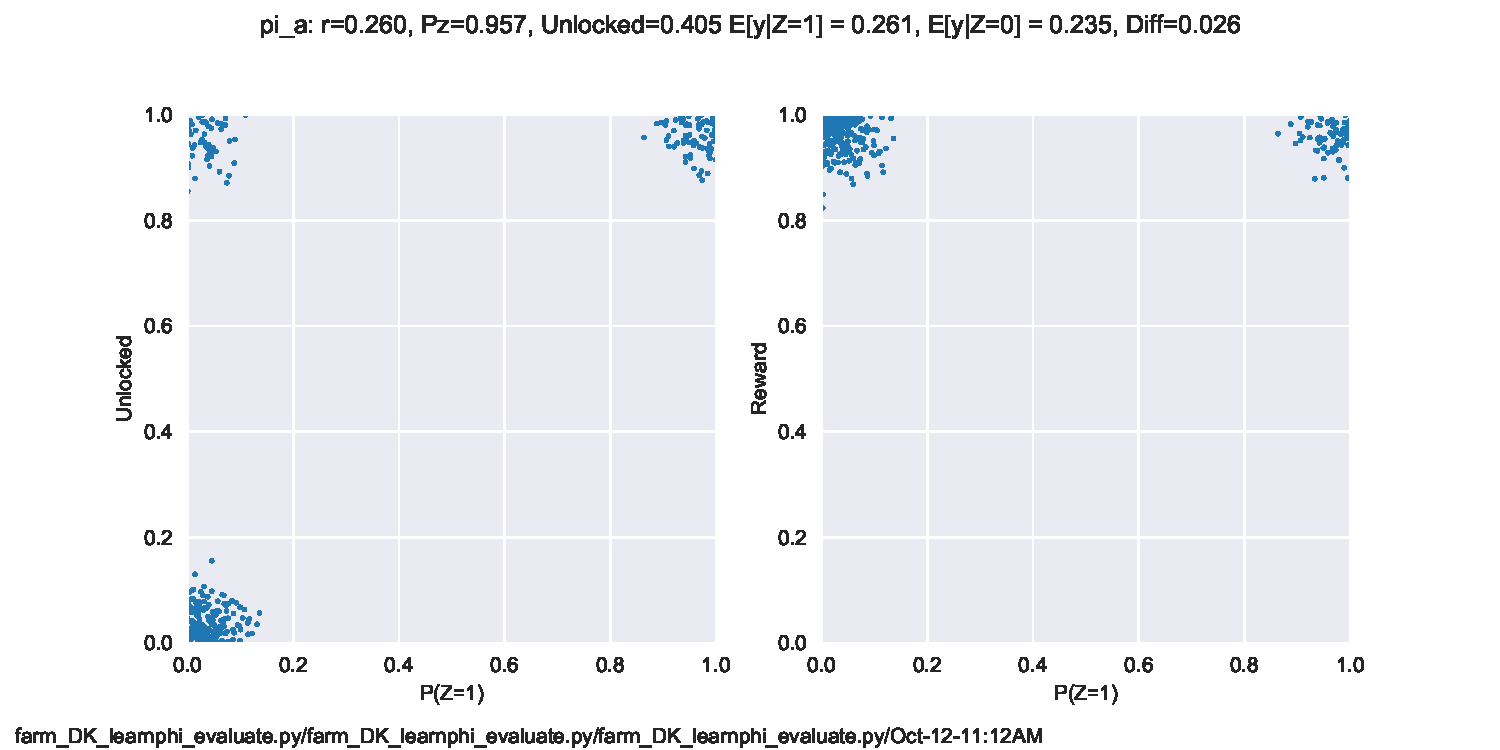
\includegraphics[width=\linewidth]{causal_figures/DK_evaluate_policy_a_c13}
%	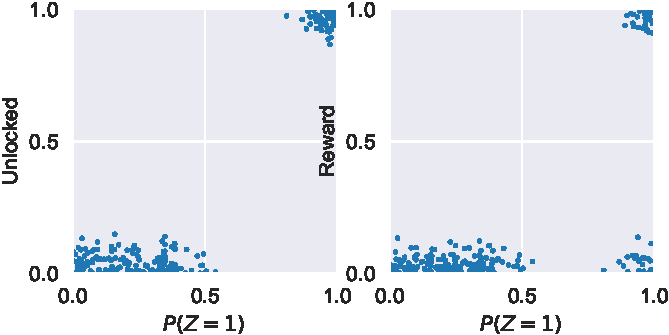
\includegraphics[width=0.9\linewidth]{causal_figures/scatter_AB}
%	%	\includegraphics[width=\linewidth]{causal_figures/scatter_cross_DK5_learnphi_AB_a_c19}		
%	\caption{Scatter plot of $P(Z=1)$ and (left) chance of unlocking the door, and (right) chance of successfully reaching the goal state. The causal variable $Z$  appears to correspond to opening the door. }\label{fig11} % also b, c. 
%\end{figure}
%    
%\end{frame}